\documentclass{report}

\usepackage{listings}
\usepackage[vlined, boxed]{algorithm2e}
\usepackage{tikz}
\usepackage{hyperref}
\usepackage{float}
%\usepackage{geometry}
\usepackage{mathtools}
\usepackage{amssymb}
\usepackage{galois}
\usepackage{titlesec}
\usepackage{stmaryrd}
\usepackage{fancyvrb}

\titleformat{\chapter}[hang]
  {\normalfont\huge\bfseries}   % formatting for chapter title (font size, style)
  {\thechapter.}                % the label (chapter number followed by a period)
  {1em}                         
  {}
\titlespacing*{\chapter}{0pt}{0pt}{20pt}

\SetAlCapSkip{2mm}

%\bibliographystyle{apalike}

\title{Implementation and Evaluation of the FunArray\\[1em]\large{}Bachelor's Thesis\\[1em]Software and Computational Systems Lab\\Ludwig-Maximilians-Universit\"at M\"unchen}
\date{September 2024}
\author{Maximilian Hofstetter}
%\institute{Software and Computational Systems Lab\\Ludwig-Maximilians-Universit\"at M\"unchen}
%\subtitle{Bachelor's Thesis}

\newcommand{\funArray}[1]{$#1$}
\newcommand{\bound}[1]{\{#1\}}
\newcommand{\fvalue}[1]{\;#1\;}



\begin{document}

\maketitle

\chapter{Introduction}
\chapter{Background}
\section{Program semantics}

Consider the following computer program written in some simple fictive programming language.

\begin{center}
\begin{BVerbatim}
i := 0;
while (i < 10) {
    i := i + 1;
}
\end{BVerbatim}
\end{center}

An experienced programmer might be quick to think they know what this code is supposed to do. They however can only see the syntax of this program and have no knowledge of what the statements actually do in the made-up language. To discover what is happening we first must define the language's semantics. 


\subsection{Environments and Expressions}

Determining the meaning of a particular statement requires us to know the current state of the program. The expression \texttt{i + 1} has an entirely different result, depending on the value of the variable \texttt{i}, which is recorded in the program's concrete scalar variable environment. An environment is defined as a function $\rho\in\mathcal{R}_v$ with $\mathcal{R}_v \triangleq \mathbb{X}\mapsto\mathcal{V}$, where $\mathbb{X}$ is the set of syntactical variable names and $\mathcal{V}$ is the set of values they can take \cite{cousot2011}.

Now consider the simple syntactical expression $\mathtt{e}\in\mathbb{E}$. It only contains scalar constants, scalar variable references and operators. Now $\llbracket\mathtt{e}\rrbracket\rho$ describes the semantics of \texttt{e} in the concrete variable environment $\rho$. The semantics of a variable \texttt{i} is defined as $\llbracket\mathtt{i}\rrbracket\rho=\rho(\mathtt{i})$ and the semantics of a syntactic operator $\circledast$ is defined as $\llbracket\mathtt{e_0\circledast e_1}\rrbracket\rho=\llbracket\mathtt{e_0}\rrbracket\rho \ast\llbracket\mathtt{e_1}\rrbracket\rho$ \cite{scott1971}. 
Imagine a variable environment $\rho$, where $\rho(\mathtt{i})=1$, for example. Our previously mentioned expression \texttt{i + 1} evaluates to:

\begin{equation*}
\begin{aligned}
\llbracket\mathtt{i \;\texttt{+}\; 1}\rrbracket\rho &=\llbracket\mathtt{i}\rrbracket\rho +\llbracket\mathtt{1}\rrbracket\rho \\
& = \rho(\mathtt{i}) + 1\\
& = 1+1\\
& = 2
\end{aligned}
\end{equation*}


\subsection{Transformers}
A computer program not only contains expressions, but also commands or statements that modify the environment itself. For example, consider the environment $\rho$ where $\rho(\mathtt{i})=1$. After executing the command \texttt{i := i + 1}, the value of the variable \texttt{i} changes and therefore the environment $\rho'$ after the execution of the command is different from $\rho$. We write $\llbracket \texttt{i\;:=\;i\;+\;1} \rrbracket\rho=\rho[\mathtt{i}:=\texttt{i\;+\;1}]=\rho'$, meaning the semantics of the environment $\rho$ after executing an assignment \texttt{i\;:=\;i\;+\;1} is an environment $\rho'$ where all occurrences of \texttt{i} have been replaced by \texttt{i\;+\;1}.

More generally the semantics of an assignment is defined as $\llbracket \texttt{i\;:=\;e} \rrbracket\rho=\rho[\mathtt{i}:=\texttt{e}]$ with $\rho[\mathtt{i}:=\texttt{e}](\mathtt{i})=\llbracket\mathtt{e}\rrbracket\rho$ \cite{cousot2011}. Commands that alter the environment are called transformations. They are basically functions in $\mathcal{R}_v\mapsto\mathcal{R}_v$ \cite{scott1971}.


\section{Abstract Interpretation}

Let us take a look at the equation $8174+2938=x$. We want to determine whether $x$ has a positive or a negative value. Instead of doing mental arithmetic and actually adding $2938$ to $8174$ we almost instinctively know that $x$ must be positive because both its summands are positive. Without realising it, we abstracted the operands of the equation to its sign and calculated it with only this property. When applied to static code analysis, this strategy we just instinctively applied, is called abstract interpretation. Its main idea is that for proving a program's properties it is not necessary to run it with concrete values. Instead it can be run on the examined properties \cite{cousot2023, cousot1977}.


\subsection{Properties}

Consider a set of entities $\mathcal{E}$. A formal property $P\subseteq \wp(\mathcal{E}) $ is a set of entities that have this property \cite[chapter 8]{cousot2021}. With the set of integers as our set of entities $\mathcal{E}=\mathbb{Z}$, our ``positive'' property is defined as $P_{pos}=\{z\in \mathcal{E} \;|\; 0<z\}$ and we can define some more semantic properties like in table \ref{table:properties}.
\begin{table}[hbt]
\begin{center}
  \begin{tabular}{l|l}
  $\mathsf{false}$ & $\emptyset$\\
   $P_{0}$ & $\{0\}$\\
   $P_{pos}$ & $\{z\in \mathbb{Z} \;|\; 0<z\}$\\
   $P_{neg}$ & $\{z\in \mathbb{Z} \;|\; 0>z\}$\\
   $P_{pos0}$ & $\{z\in \mathbb{Z} \;|\; 0\leq z\}$\\
   $P_{neg0}$ & $\{z\in \mathbb{Z} \;|\; 0\geq z\}$\\
   $P_{even}$ & $\{z\in \mathbb{Z} \;|\; \exists k\in\mathbb{Z}:2k=z \}$ \\
   $P_{odd}$ & $\{z\in \mathbb{Z} \;|\; \exists k\in\mathbb{Z}:2k+1=z \}$ \\
   $P_{pos\_even}$ & $\{z\in \mathbb{Z} \;|\; z>0 \wedge \exists k\in\mathbb{Z}:2k=z \} = P_{pos} \cap P_{even}$ \\
   $\vdots$ &$\vdots$\\
   $\mathsf{true}$ & $\mathbb{Z}$\\
  \end{tabular}
  \caption{An incomplete selection of properties for $\mathbb{Z}$.}\label{table:properties}
  \end{center}
\end{table}

We call a property $P$ ``stronger'' than $P'$ (or $P'$ ``weaker'' than $P$) if $P\subseteq P'$. Its set representation contains less elements and we therefore have more information about an element that fulfils said property. The weakest property is the $\mathsf{true}$ property that is satisfied by alle elements and the strongest is $\mathsf{false}$ which is satisfied by none \cite[chapter 8]{cousot2021}. Not all properties from $\wp(\mathcal{E})$ carry a semantic meaning. We therefore only consider the set of properties of interest $C\subseteq\wp(\mathcal{E})$. If we want to analyse the signs of integers this could be $C_{sign}=\{\mathsf{false}, P_{0}, P_{pos}, P_{neg}, P_{pos0}, P_{neg0}, P_{not0}, \mathsf{true}\}$. The poset  $\langle C,\subseteq\rangle$ is called the ``concrete domain''.

\subsection{Abstraction}

Now consider a set of abstract properties $A$. This is not a power set of concrete values anymore but a set of purely semantic symbols that represent abstract properties. If there exists a Galois connection $\langle C,\subseteq\rangle \galois{\alpha}{\gamma}\langle A\sqsubseteq\rangle$, we call $\langle A\sqsubseteq\rangle$ the abstract domain, $\alpha\in C\to A$ the abstraction function and $\gamma\in A\to C$ the concretisation function \cite[chapter 11]{cousot2021}. To put the working principle of Galois connections into simple terms: $A$'s elements abstract $C$'s elements and $\sqsubseteq$ works analogous in the abstract to $\subseteq$ in the concrete. More formally: $\forall P_C\in C:\forall P_A \in A:\alpha(P_C)\sqsubseteq P_A \Longleftrightarrow P_C \subseteq \gamma(P_A)$.

\begin{figure}[htb]
	\begin{center}
		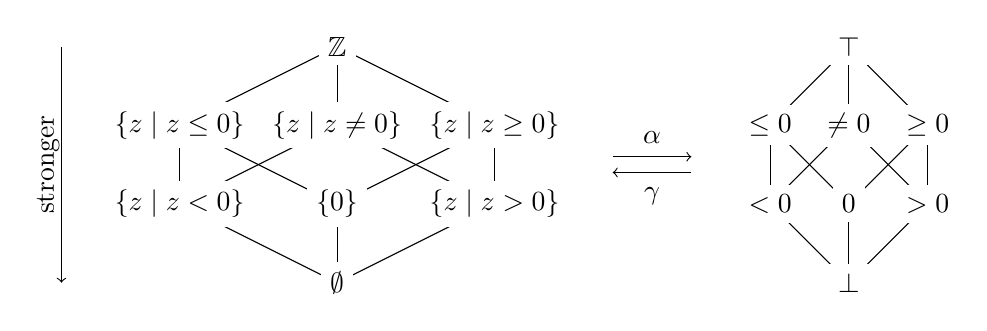
\begin{tikzpicture}
			% Concrete domain
			\draw (-4.5,0) -- (-6.5,1);
            \draw (-4.5,0) -- (-4.5,1);
            \draw (-4.5,0) -- (-2.5,1);
            \draw (-4.5,3) -- (-6.5,2);
            \draw (-4.5,3) -- (-4.5,2);
            \draw (-4.5,3) -- (-2.5,2);
            
            \draw (-4.5,1) -- (-6.5,2);
            \draw (-4.5,1) -- (-2.5,2);
            \draw (-6.5,1) -- (-6.5,2);
            \draw (-2.5,1) -- (-2.5,2);
            \draw (-4.5,2) -- (-6.5,1);
            \draw (-4.5,2) -- (-2.5,1);
            
            \draw (-4.5,0) node[fill=white!5] {$\emptyset$};
            \draw (-6.5,1) node[fill=white!5] {$\{z\;|\;z<0\}$};
            \draw (-4.5,1) node[fill=white!5] {$\{0\}$};
            \draw (-2.5,1) node[fill=white!5] {$\{z\;|\;z>0\}$};
            \draw (-6.5,2) node[fill=white!5] {$\{z\;|\;z\leq0\}$};
            \draw (-4.5,2) node[fill=white!5] {$\{z\;|\;z\neq0\}$};
            \draw (-2.5,2) node[fill=white!5] {$\{z\;|\;z\geq0\}$};
            \draw (-4.5,3) node[fill=white!5] {$\mathbb{Z}$};

			% Abstract domain
            \draw (2,0) -- (1,1);
            \draw (2,0) -- (2,1);
            \draw (2,0) -- (3,1);
            \draw (2,3) -- (1,2);
            \draw (2,3) -- (2,2);
            \draw (2,3) -- (3,2);
            
            \draw (2,1) -- (1,2);
            \draw (2,1) -- (3,2);
            \draw (1,1) -- (1,2);
            \draw (3,1) -- (3,2);
            \draw (2,2) -- (1,1);
            \draw (2,2) -- (3,1);
            
            \draw (2,0) node[fill=white!5] {$\perp$};
            \draw (1,1) node[fill=white!5] {$<0$};
            \draw (2,1) node[fill=white!5] {$0$};
            \draw (3,1) node[fill=white!5] {$>0$};
            \draw (1,2) node[fill=white!5] {$\leq0$};
            \draw (2,2) node[fill=white!5] {$\neq0$};
            \draw (3,2) node[fill=white!5] {$\geq0$};
            \draw (2,3) node[fill=white!5] {$\top$};
            
            
            % Arrows
            \draw (-0.5,1.85) node {$\alpha$};
            \draw [->](-1,1.6) -- (0,1.6);
            \draw [<-](-1,1.4) -- (0,1.4);
            \draw (-0.5,1.1) node {$\gamma$};
            
            \draw [<-](-8,0) -- (-8,3);
            \draw (-8.17,1.5) node[rotate=90] {stronger};
        \end{tikzpicture}
        \caption{The sign properties of the concrete integer domain (left) next to the abstract sign domain (right) as a Hasse diagram. }
	\end{center}
\end{figure}

\subsection{Property Transformers}


\subsection{Fixpoint analysis}

\subsection{The Interval Domain}
asdf

\begin{figure}[htb]
	\begin{center}
		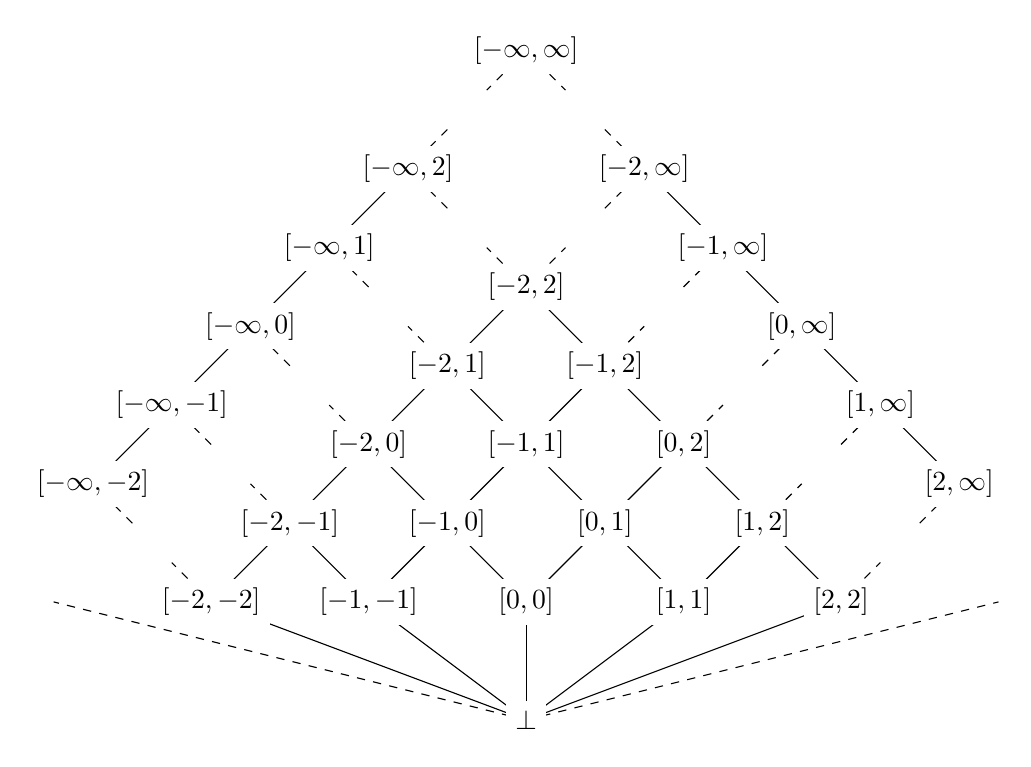
\begin{tikzpicture}
            \draw (0,0) -- (0,1.5);
            \draw (0,0) -- (2,1.5);
            \draw (0,0) -- (4,1.5);
            \draw (0,0) -- (-2,1.5);
            \draw (0,0) -- (-4,1.5);
            \draw (0,0)[dashed] -- (-6,1.5);
            \draw (0,0)[dashed] -- (6,1.5);
            
            \draw (2,1.5) -- (1,2.5);
            \draw (2,1.5) -- (3,2.5);
            \draw (4,1.5) -- (3,2.5);
            \draw (0,1.5) -- (1,2.5);
            \draw (0,1.5) -- (-1,2.5);
            \draw (-2,1.5) -- (-1,2.5);
            \draw (-2,1.5) -- (-3,2.5);
            \draw (-4,1.5) -- (-3,2.5);
            
            \draw (1,2.5) -- (0,3.5);
            \draw (1,2.5) -- (2,3.5);
            \draw (3,2.5) -- (2,3.5);
            \draw (-1,2.5) -- (0,3.5);
            \draw (-1,2.5) -- (-2,3.5);
            \draw (-3,2.5) -- (-2,3.5);
            
            \draw (2,3.5) -- (1,4.5);
            \draw (0,3.5) -- (1,4.5);
            \draw (0,3.5) -- (-1,4.5);
            \draw (-2,3.5) -- (-1,4.5);
            
            \draw (-1,4.5) -- (0,5.5);
            \draw (1,4.5) -- (0,5.5);
            
            \draw (-4,1.5)[dashed] -- (-4.5,2);
            \draw (-5,2.5)[dashed] -- (-5.5,3);
            
            \draw (-3,2.5)[dashed] -- (-3.5,3);
            \draw (-4,3.5)[dashed] -- (-4.5,4);
            
            \draw (-2,3.5)[dashed] -- (-2.5,4);
            \draw (-3,4.5)[dashed] -- (-3.5,5);
            
            \draw (-1,4.5)[dashed] -- (-1.5,5);
            \draw (-2,5.5)[dashed] -- (-2.5,6);
            
            \draw (0,5.5)[dashed] -- (-0.5,6);
            \draw (-1,6.5)[dashed] -- (-1.5,7);
           
            \draw (4,1.5)[dashed] -- (4.5,2);
            \draw (5,2.5)[dashed] -- (5.5,3);
            
            \draw (3,2.5)[dashed] -- (3.5,3);
            \draw (4,3.5)[dashed] -- (4.5,4);
            
            \draw (2,3.5)[dashed] -- (2.5,4);
            \draw (3,4.5)[dashed] -- (3.5,5);
            
            \draw (1,4.5)[dashed] -- (1.5,5);
            \draw (2,5.5)[dashed] -- (2.5,6);
            
            \draw (0,5.5)[dashed] -- (0.5,6);
            \draw (1,6.5)[dashed] -- (1.5,7);
            
            \draw (-5.5,3) -- (-1.5,7);
            \draw (5.5,3) -- (1.5,7);
            
            \draw (-1,7.5)[dashed] -- (-1.5,7);
            \draw (1,7.5)[dashed] -- (1.5,7);
            
            \draw (0,8.5)[dashed] -- (-0.5,8);
            \draw (0,8.5)[dashed] -- (0.5,8);
            
            \draw (0,0) node[fill=white!5] {$\perp$};
            \draw (0,1.5) node[fill=white!5] {$[0,0]$};
            \draw (2,1.5) node[fill=white!5] {$[1,1]$};
            \draw (4,1.5) node[fill=white!5] {$[2,2]$};
            \draw (-2,1.5) node[fill=white!5] {$[-1,-1]$};
            \draw (-4,1.5) node[fill=white!5] {$[-2,-2]$};
            
            \draw (1,2.5) node[fill=white!5] {$[0,1]$};
            \draw (3,2.5) node[fill=white!5] {$[1,2]$};
            \draw (-1,2.5) node[fill=white!5] {$[-1,0]$};
            \draw (-3,2.5) node[fill=white!5] {$[-2,-1]$};
            
            \draw (2,3.5) node[fill=white!5] {$[0,2]$};
            \draw (0,3.5) node[fill=white!5] {$[-1,1]$};
            \draw (-2,3.5) node[fill=white!5] {$[-2,0]$};
            
            \draw (1,4.5) node[fill=white!5] {$[-1,2]$};
            \draw (-1,4.5) node[fill=white!5] {$[-2,1]$};
            
            \draw (0,5.5) node[fill=white!5] {$[-2,2]$};
            
            
            \draw (-5.5,3) node[fill=white!5] {$[-\infty,-2]$};
            \draw (-4.5,4) node[fill=white!5] {$[-\infty,-1]$};
            \draw (-3.5,5) node[fill=white!5] {$[-\infty,0]$};
            \draw (-2.5,6) node[fill=white!5] {$[-\infty,1]$};
            \draw (-1.5,7) node[fill=white!5] {$[-\infty,2]$};
            
            
            \draw (5.5,3) node[fill=white!5] {$[2,\infty]$};
            \draw (4.5,4) node[fill=white!5] {$[1,\infty]$};
            \draw (3.5,5) node[fill=white!5] {$[0,\infty]$};
            \draw (2.5,6) node[fill=white!5] {$[-1,\infty]$};
            \draw (1.5,7) node[fill=white!5] {$[-2,\infty]$};
            
            \draw (0,8.5) node[fill=white!5] {$[-\infty,\infty]$};
         
        \end{tikzpicture}
        \caption{The interval abstract domain as a Hasse diagram \cite{cousot1977}}.\label{fig:intervaldomain}
	\end{center}
\end{figure}

\section{FunArray}
\subsection{Functors}
\subsection{Abstractions}
\subsection{Segmentation Functor: The FunArray}




\chapter{Implementation}

\section{Scalar Variables}
\subsection{Intervals}
\subsection{Signs}
\section{FunArray}
\subsection{Unifying two FunArrays}
\section{Expressions}
\subsection{Evaluation of an Expression}
\subsection{Normalisation of an Expression}
\section{Statements}



\chapter{Evaluation}
\textcolor{red}{-- Forschungsfragen nochmal aufgreifen}

To evaluate 

\section{Experimental Setup}
\subsection{Benchmarks}

The International Competition on Software Verification (or SV-COMP)\footnote{More information about SV-COMP available at \url{https://sv-comp.sosy-lab.org/}} provides a set of benchmarks that can be used to compare tools for software verification\footnote{Available at \url{https://gitlab.com/sosy-lab/benchmarking/sv-benchmarks}}. Their subcategory \textit{c/ReachSafety-Arrays} contains a collection of 433 verification tasks written in C for which the treatment of arrays is necessary to determine reachability. As such, this collection is suitable to test my implementation of the FunArray. They include at least one assertion per benchmark and its expected verdict for testing 
The simple C programs have been translated to the embedded domain-specific language in Java using the tool Cuv\'ee \cite{ernst2020}. Since my implementation of the FunArray does not provide the entire functionality of the C language, about half of the benchmarks could not be translated. The 196 untranslatable benchmarks utilise features like the use of boolean variables, nested arrays, functions with a return value, structs and the use of the break keyword.

\subsection{Formal Arguments of the FunArray}

One of the FunArray's strengths is its ability to use different abstract domains for its bounds, array elements and variables without having to adapt the static analyser. For this evaluation the following abstract domains have been chosen as the FunArray functor's formal arguments: For abstracting variables and array elements the interval domain has been chosen, since it is relatively simple to implement. The chosen expression domain and therefore the abstract representation of segment bounds follows the scheme used by the FunArray's inventors \cite[section 7.2]{cousot2011}. Expressions are limited to the normal form $v+k$ where $v$ is a variable (whose value is abstracted by intervals) and $k$ is an integer constant.

\section{Results}

The execution time of the benchmarks is almost negligible. To execute all 237 benchmarks it takes 253 milliseconds (Averaged value over 100 runs. The workbench used is a M2 Max MacBook Pro running OpenJDK 22). This comes down to about a millisecond per benchmark. This result was expected, since the FunArray does not handle disjunctions separately but through the use of empty segments. No combinatorial explosion can occur.

\subsection{Invariants}
Spread across the 238 benchmarks there are 947 loops. For 580 or 61.3\% of those my implementation of the FunArray was able to determine a non-trivial invariant. A non-trivial invariant is defined as a state in which at least one of the arrays contains a segment whose value is not $\top$.
This definition of non-triviality, however, does not take the FunArrays ability to depict multiple segments into account. If we were to treat all arrays as a single segment with a homogenous value across all elements, we could have gotten the same result and the same number of non-trivial invariants. We therefore narrow down the non-triviality criterion to those states containing at least one array with more than one segment and at least one segment with a value that is not $\top$. Now we arrive at 427 non-trivial invariants, which is still 45.0\%. 
If we were to increase the required number of segments to more than two, this number would drop down to 3, suggesting the FunArrays ability to depict a lot of segments cannot be utilised in actual code analyses. No calculated invariants had more than three segments.

\subsection{Verifying assertions}

My implementation is able to correctly identify the result of 24 out of the 247 assertions spread among 237 benchmarks or 9.7\% of assertions. When manually inspecting the program mechanism preceding these assertions in the benchmark, a single pattern can be identified that precedes the majority of them: Initialisation. The benchmark first initialises an array with a consistent value as its every element and immediately afterwards asserts that every element of the array has that specific value. Of the 24 correctly assessed assertions, 20 follow this pattern. The remaining four assertions follow a more complex program scheme, that involves conditions and loops.



\section{Discussion}
\subsection{Comparison with Cousot, Cousot and Logozzo's Results}

Cousot, Cousot and Logozzo evaluate their implementation of the FunArray by analysing the main libraries of the .NET framework and the implementation itself \cite{cousot2011}. The .NET libraries have been chosen for this since they contain a large amount of code and a vast selection of functionalities and techniques. They, however, lack an important aspect: The specification of expected properties. The authors are able to infer thousands of invariants but cannot determine whether they actually provide any useful information for the further execution of the code. To check against pre-specified properties they annotated their implementation of the FunArray with pre-conditions and proof obligations and ran it on itself. They were able to correctly assert 61 out of 1800 or 3.4\% of proof obligations when analysing the FunArray implementation using itself \cite{cousot2011}. This roughly matches my results of 9.7\%, considering the easy initialisation assertions make up a way greater amount of my test cases than would be present in a real world program.

\subsection{Limitations}

\subsubsection{Adjacent potentially empty segments}
When expanding a segment by inserting a value adjacent to it, formerly adjacent and potentially empty segments will be joined with their nearest neighbour until a non-empty segment is reached. Let us consider the FunArray \funArray{A:\bound{a} \fvalue{x} \bound{b} \fvalue{y} \bound{c}? \fvalue{z} \bound{d}} for example. It is unknown whether its second segment containing the value $y$ is empty or not and thus whether $b=c$ or $b<c$ is true.

When trying to expand the first segment by inserting its value $x$ at index $b$, the resulting FunArray could either be \funArray{\bound{a} \fvalue{x} \bound{b\;c} \fvalue{x} \bound{b+1}? \fvalue{z} \bound{d}}, if the $y$-segment was empty, or alternatively \funArray{\bound{a} \fvalue{x} \bound{b} \fvalue{x} \bound{b+1} \fvalue{y} \bound{c}? \fvalue{z} \bound{d}}, if it was non-empty. Since the position of the \funArray{\bound{c}}-bound cannot by decided, it must be discarded altogether. After the insertion, $A$ becomes \funArray{A':\bound{a} \fvalue{x} \bound{b} \fvalue{x} \bound{b+1}? \fvalue{y\sqcup z} \bound{d}} and all information concerning the variable $c$ is lost.

 Analyses of programs utilising segments in their arrays with adjacent and potentially empty segments have to discard non-trivial information. Thus the FunArray's approach for handling potentially empty adjacent segments limits the number of programs for which an analysis can achieve a non-trivial result.
 
 Consider Algorithm \ref{algo:dijkstra}, Dijkstra's Dutch national flag algorithm, for example. Even though the analysis correctly determines the Array to be described as $\bound{0} \fvalue{[-\infty, -1]} \bound{r}? \fvalue{\top} \bound{w}? \fvalue{[0, 0]} \bound{b}? \fvalue{[1, \infty]}  \bound{|A|}?$ after a single loop pass, it loses all its information in the second pass, because the determined segments are all potentially empty and extending their neighbours discards them altogether. After the second loop pass the analysis yields $\bound{0} \fvalue{\top} \bound{|A|}$. Basically no information can be gained   
 
\vspace{2mm}
\begin{algorithm}[H]
$r \leftarrow 0$\\
$w,b \leftarrow$ length of $A-1$ \\
\vspace{1.5mm}
\While{ $r\leq w$}{
    \vspace{0.7mm}
    \vspace{0.7mm}
    \If{$A[w]\leq -1$}{
        \vspace{0.7mm}
        switch values of $A[w]$ and $A[r]$\\
        $r\leftarrow r+1$ 
    }
    \vspace{1mm}
    \If{$A[w]=0$ }{
        \vspace{0.7mm}
        $w\leftarrow w-1$
    }
    \vspace{1mm}
    \If{$A[w]\geq1$}{
        \vspace{0.7mm}
        switch values of $A[w]$ and $A[b]$\\
        $w\leftarrow w-1$ \\
        $b\leftarrow b-1$ 
    }
}
\end{algorithm}


\chapter{Conclusion}

Strength: Initialization of Arrays




\newpage
\bibliographystyle{plain}
\bibliography{Bibliography}
\end{document}